\newpage
\section{Auswertung}
Das gegebene Matlab Skript 'Skript.m' wurde gemäß der Versuchsanleitung \cite[S. 11]{Laboranleitung} erweitert.
Zuerst wurde der gegebene Datensatz 'Datensatz.m' überarbeitet und in die Struktur ts zusammengefasst, um ein übersichtlicheres Arbeiten in Matlab zu ermöglichen.
Dieser veränderte Datensatz wurde als 'DatensatzModified.m' abgespeichert und im restlichen verlauf der Durchführung verwendet.


\subsection{Vergleich der Leistungsflüsse}
Der Vergleich zwischen den simulierten und gemessenen Leistungen wurde mittels der Plot-Funktion in \autoref{fig:plot_230730} dargestellt,
dabei wurden zur Übersichtlichkeit zusätzlich Kurzzeitmittelwerte gebildet um einen Leistungsverlauf in Minutenwerten darzustellen.

\begin{figure}[H]
    \centering
    \includegraphics[width=\textwidth]{Abbildungen/leistungsflüsse.jpg}
    \caption{Vergleich der Leistungsflüsse}
    \label{fig:plot_230730}
\end{figure}

\newpage
Auffälligkeiten beziehungsweise Abweichungen zwischen realem und simuliertem Leistungsfluss zeigen sich in verschiedenen Zeiträumen.
Der Zeitraum des 19. Juli (\autoref{fig:plot_230731}) wurde ausgesucht, um eventuelle Fehlerquellen zu identifizieren. Es können zwei Zeiträume identifiziert werden in denen starke Abweichungen zwischen Real- und Simulationswerten entsteht. Zwischen 8 Uhr und 9 Uhr morgens wird ein Ladezustand der Batterie simuliert, tatsächlich wird diese jedoch erst ab ca. 9.10 Uhr geladen. Am Nachmittag zwischen 14 und 15 Uhr wird die Batterie weiterhin geladen, während kein Leistungsfluss simuliert wird.


\begin{figure}[H]
    \centering
    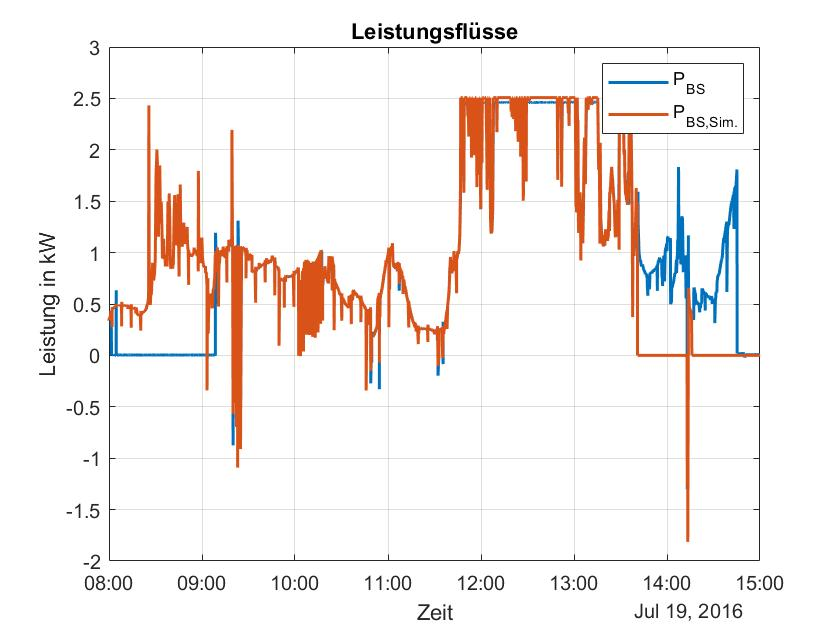
\includegraphics[width=1\textwidth]{Abbildungen/8.15.jpg}
    \caption{Vergleich der Leistungsflüsse in einem ausgesuchten Zeitraum}
    \label{fig:plot_230731}
\end{figure}

Die Abweichungen zwischen simulierten und realen Werten kommt zustande, da das simulierte System sofort reagiert, was beim realen System nicht möglich ist. Dies lässt sich in \autoref{fig:plot1_230731} gut erkennen.
\begin{figure}[H]
    \centering
    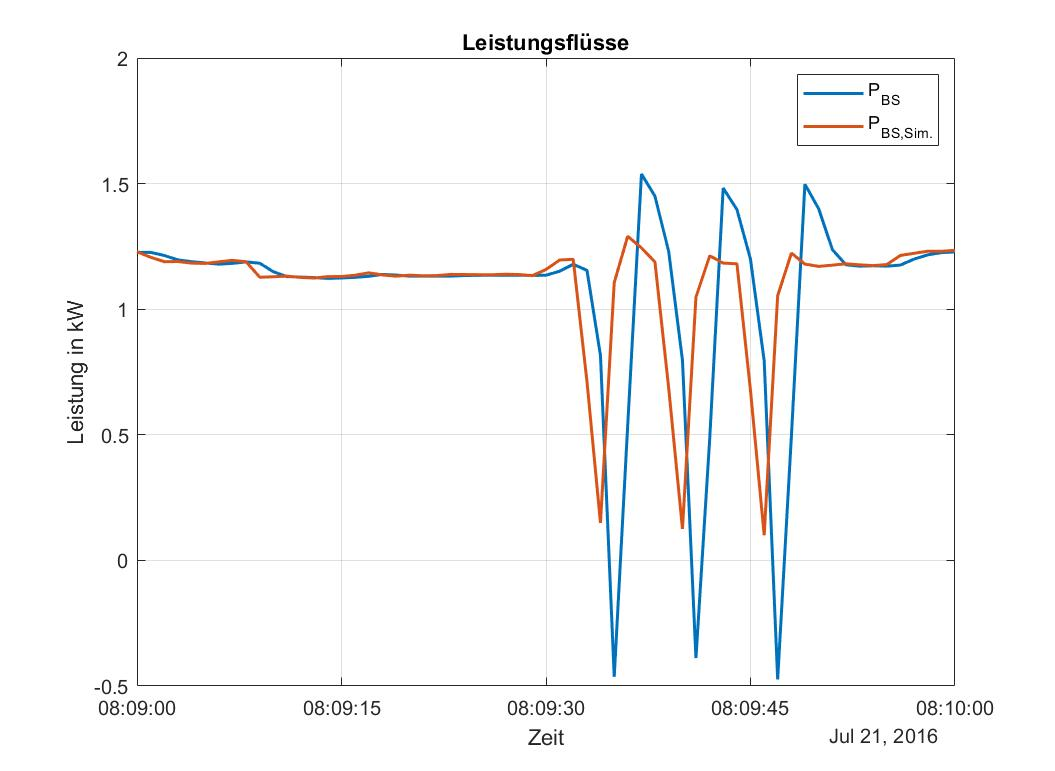
\includegraphics[width=0.95\textwidth]{Abbildungen/8.09.jpg}
    \caption{Vergleich der Leistungsflüsse}
    \label{fig:plot1_230731}
\end{figure}

In \autoref{fig:plot2_230731} ist erkenntlich, dass auf einen relativ großen Simulationsfehler viele kleinere Folgefehler folgen können, da das System versucht den ersten auszugleichen.

\begin{figure}[H]
    \centering
    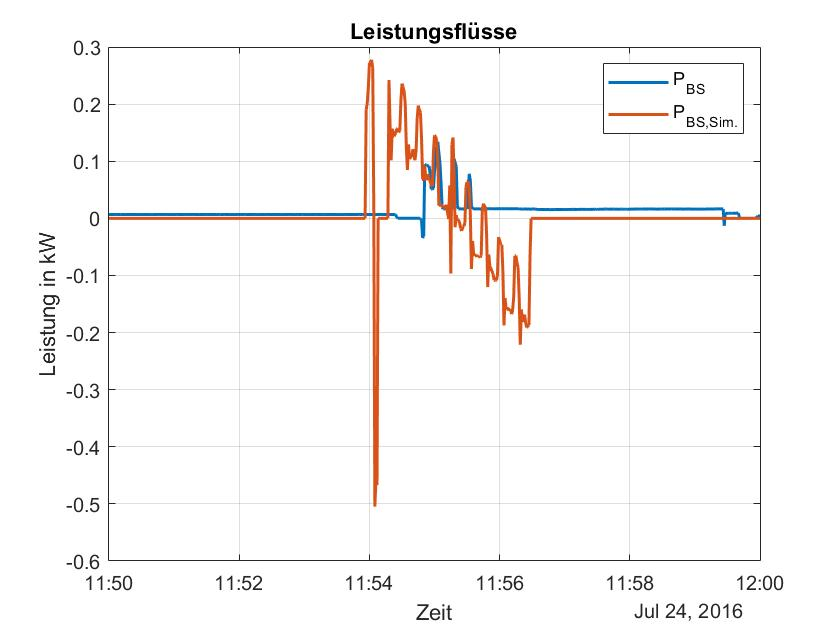
\includegraphics[width=0.95\textwidth]{Abbildungen/11.54.jpg}
    \caption{Vergleich der Leistungsflüsse}
    \label{fig:plot2_230731}
\end{figure}


Das Streudiagramm wurde mit der Scatter-Funktion erstellt und in \autoref{fig:plot1_230730_1} dargestellt und soll ein Verständnis zum Betriebsverhalten des Batteriesystems vermitteln. Jeder Punkt stellt einen sekündlichen Wert der Messzeit über 7 Tage dar.
\begin{figure}[H]
    \centering
    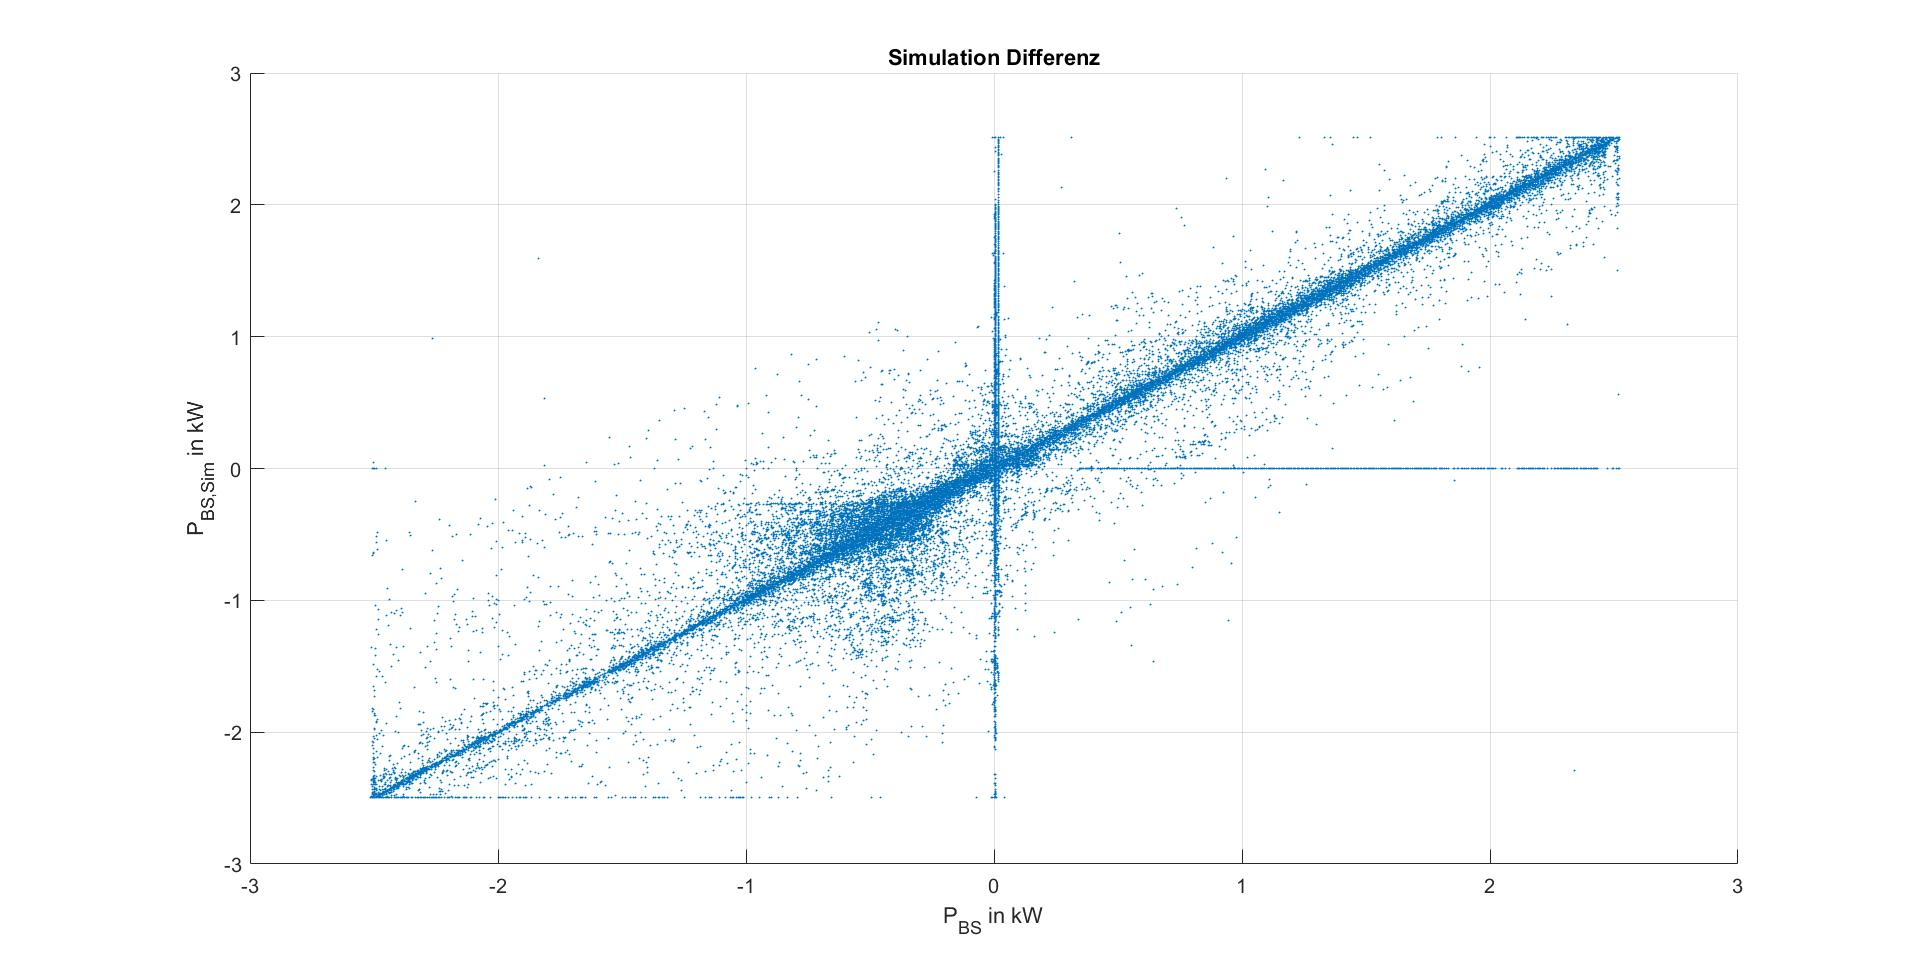
\includegraphics[width=\textwidth]{Abbildungen/streudiagramm.jpg}
    \caption{Streudiagramm}
    \label{fig:plot1_230730_1}
\end{figure}



Die Linie der Gleichheit verläuft diagonal vom dritten in den zweiten Quadranten und ist klar erkennbar. Wäre die Simulation identisch mit den realen Werten, so würden alle Punkte auf dieser Diagonalen liegen. Das lässt schlussfolgern, dass die Simulation mit den realen Werten in vielen Punkten übereinstimmt, jedoch nicht in allen.
Klar zu erkennen sind die Grenzen des Systems bei 2,5 kW beziehungsweise -2,5 kW welche durch die maximale Lade- und Entladeleistung definiert werden.

Besondere Abweichungen lassen sich an den zwei Nullinien erkennen. Die Gerade zwischen dem 1. und 4. Quadranten zeigt Abweichungen zwischen den realen Werten welche steigen während die simulierten Werte bei null bleiben. Die senkrechte Linie auf der y-Achse beschreibt das Gleiche nur umgekehrt, die simulierten Werte steigen bei gleichbleibenden Realen. Dieser Effekt beruht wie im vorherigen Kapitel beschrieben auf den verschiedenen Reaktionszeiten der beiden Systeme. 
Also Beispielsweise darauf, dass die Simulation bereits eine Leistung aufnimmt, bevor das reale System überhaupt angefangen hat oder das reale System noch Leistungsflüsse ausführt, die im idealen schon beendet wurden.
Besondere Streuungen sind außerdem im 3. Quadranten zwischen -1 und 0 zu erkennen, was durch das dynamische Regelverhalten bei stark schwankenden Lasten erklärt werden kann. 

\subsection{Vergleich der Energiesummen}
\subsubsection{Abweichungen zwischen den kumulierten Energiesummen der gemessenen und
simulierten Energieaufnahme und -abgabe des Batteriesystems}
Die kumulierten Summen werden mithilfe des 'cumsum'-Befehls und der Plot-Funktion in \autoref{fig:plot1_230730} dargestellt.

\begin{figure}[H]
    \centering
    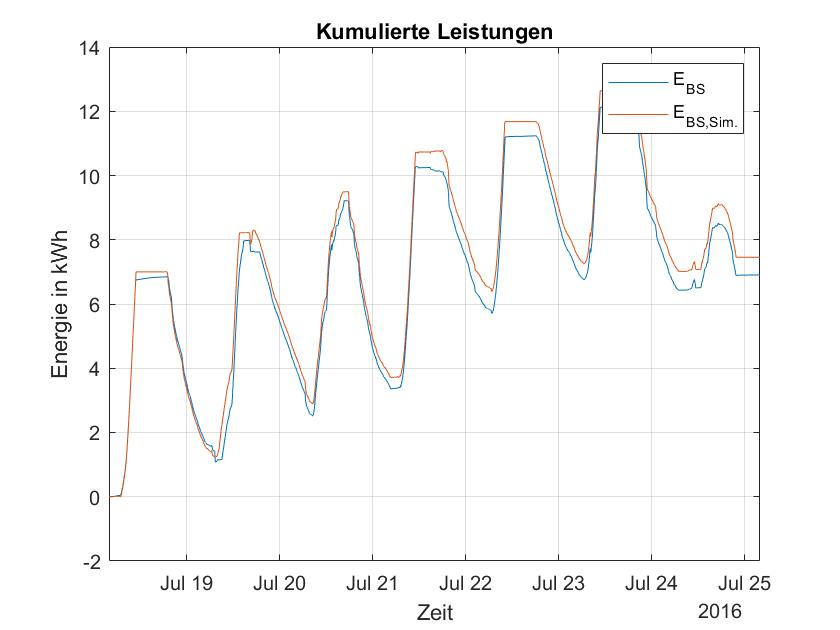
\includegraphics[width=\textwidth]{Abbildungen/kummulierteleistungen.jpg}
    \caption{Kumulierte Leistungen}
    \label{fig:plot1_230730}
\end{figure}
\newpage
Anschließend wurden sowohl die positiven wie auch die negativen Leistungsströme in \autoref{fig:plot1_230730_2} und \autoref{fig:plot1_230730_3} kummuliert dargestellt.
\begin{figure}[H]
    \centering
    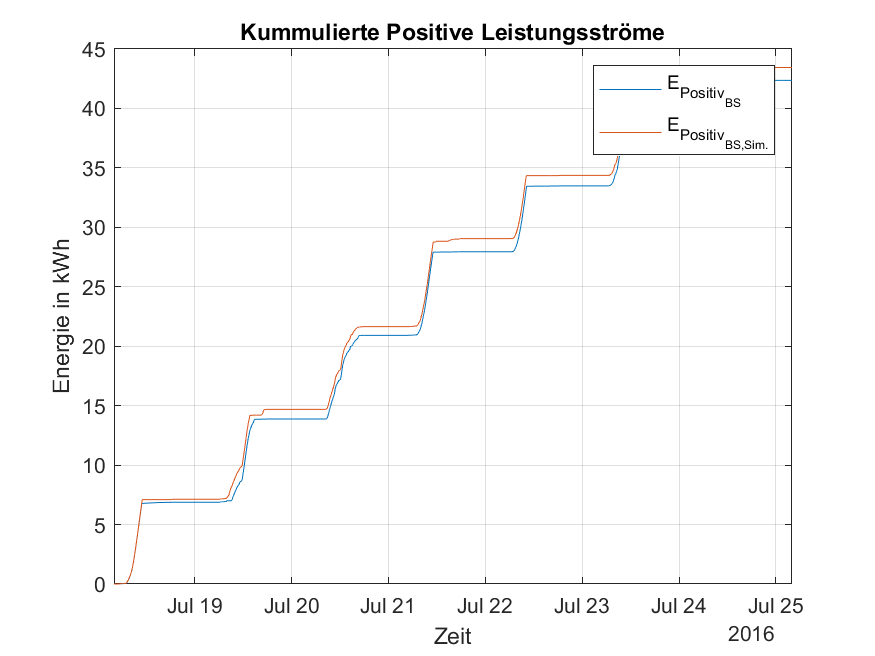
\includegraphics[width=0.87\textwidth]{Abbildungen/plot5.png}
    \caption{Kummulierte positive Leistungsströme}
    \label{fig:plot1_230730_2}
\end{figure}

\begin{figure}[H]
    \centering
    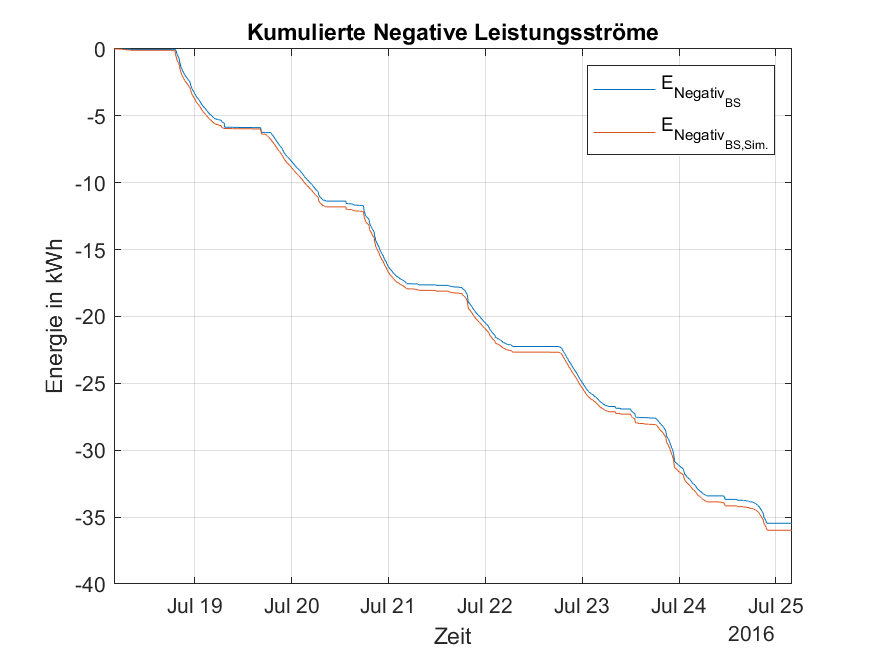
\includegraphics[width=0.87\textwidth]{Abbildungen/plot6.png}
    \caption{Kummulierte negative Leistungsströme}
    \label{fig:plot1_230730_3}
\end{figure}
Dabei ist zu sehen, dass die simulierten Werte immer größer sind als die gemessenen. Dies lässt vermuten, dass die Simulation 
nicht die tatsächlichen Verluste der Leistungs-auf und -abgabe mit Berücksichtigt. Weitere Fehlerquellen könnten dabei durch Messfehler oder eine nicht Berücksichtigung von Faktoren wie Alterung des Batteriesystems sein.\\

\subsubsection{Energiesummen, Nutzungsgrade des Batterieumrichters,
Batteriespeichers und Batteriesystems}
Die für Aufgabe 7.2.2 der Versuchsanleitung \cite[S. 11]{Laboranleitung} verlangten Werte wurden in der Struktur Ergebnisse in Matlab zusammengefasst.
Energiesummen der Leistungen lassen sich jeweils durch die Funktion cumsum() ermitteln, der absolute Fehler der Energiesummen lässt sich mit der Differenz aus den realen Energiesummen und den simulierten Energiesummen errechnen und der relative aus dem Quotienten zwischen dem absoluten Fehler und der dazugehörigen Energiesumme.
Die AC-Batterieladung wurde ermittelt, indem nur die Batterieleistungsflüsse geloggt wurden, welche größer als 0 waren.
Die Batterieentladung bildet dabei das Gegenstück und sind nur die Batterieleistungsflüsse, die kleiner als 0 waren.
Für die DC-Batterieladung und -Entladung wurde genauso vorgegangen, nur das hier die Batteriesystemleistungsflüsse verwendet wurden.
Der AC2BAT-Nutzungsgrad wurde mit $\frac{AC-Batterieladung}{DC_Batterieladung}$ berechnet, der Nutzungsgrad der Batterie mit $\frac{DC-Batterieentladung}{DC_Batterieladung}$, der BAT2AC-Nutzungsgrad mit $\frac{DC-Batterieentladung}{AC-Batterieentladung}$ und der AC-Systemnutzungsgrad mit $\frac{DC-Batterieentladung}{DC-Batterieladung}$.
\\
\begin{table}[ht!]
    \centering
    \caption{Abweichungen der Energiesummen sowie der Nutzungsgrade zwischen den Mess- und Simulationsergebnissen}
    \label{tab_Ergebnisse}
    \small
 \begin{tabular}{|l|l|l|l|l|l|}
    \hline \rowcolor[HTML]{70AD47} 
    { \textbf{Bezeichnung}} & { \textbf{Kürzel}} & { \textbf{Messung}} & {\textbf{Simulation}} & {\textbf{\makecell{absolute\\Abweichung}}} & { \textbf{\makecell{relative\\Abweichung\\ (in\%)}}} \\ \hline
    
    AC-Batterieladung in kWh                    &$E_{AC2BS}$                         & 40,46                                              & 40,95                                  & -0,498                                         & -1,23                                   \\ \hline
    
    AC-Batterieentladung in kWh                 &$E_{BS2AC}$                         & 37,22                                              & 37,96                                  & -0,741                                        & -1,99                                   \\ \hline
  
    DC-Batterieladung in kWh                    &$E_{BATC}$                          & 42,37                                              & 43,44                                  & -1,077                                        & -2,54                                   \\ \hline
   
    DC-Batterieentladung in kWh                 &$E_{BATD}$                          & 35,46                                              & 35,99                                  & -0,529                                         & -1,5                                    \\ \hline
     
    AC2BAT-Nutzungsgrad in \%                  &$\bar{\eta}_{AC2BAT}$               & 95,5                                              & 94,3                                  & 1,22                                         & 1,28                                    \\ \hline
   
    {\makecell{Nutzungsgrad\\der Batterie in \%}} &$\bar{\eta}_{BAT}$                & 92                                               & 92,7                                  & -0,69                                        & -0,75                                   \\ \hline
  
    BAT2AC-Nutzungsgrad in\%                  &$\bar{\eta}_{BAT2AC}$               & 95,3                                              & 94,8                                  & 0,47                                         & 0,49                                    \\ \hline
   
    AC-Systemnutzungsgrad in\%                &$\bar{\eta}_{AC}$                   & 83,7                                              & 82,8                                  & 0,86                                         & 1,02                                    \\ \hline
 \end{tabular}
\end{table}

Die Simulation erweist sich im Allgemeinen als sehr genau, da alle Abweichungen über den 
gesamten Messzeitraum bei maximal etwas über 2,5 \% liegen. 
Insbesondere wurde der Entladevorgang genauer simuliert als der Ladevorgang, 
was vermuten lässt, dass die Entladung verlustärmer als die Ladung des Systems ist.
Es ist anzumerken, dass die Simulation die Verluste 
nur teilweise berücksichtigt hat, und die in der Realität gemessenen Wirkungsgrade tatsächlich fast alle höher sind als in der Simulation.
\\
Um die Ursachen der Differenzen zwischen Messung und Simulation zu ermitteln, müsste man die Methode zur Berechnung der mittleren 
Wirkungsgrade in der Simulation untersuchen und 
die Unterschiede in der Nutzung, den äußeren Bedingungen wie Temperatur und Einstrahlung sowie anderen Faktoren berücksichtigen. Eine genaue Analyse dieser Aspekte könnte dabei helfen, die Abweichungen zwischen den Mess- und Simulationsdaten zu erklären.